% 固定源印刷页34；与全国文第21题相同题设的斜棱平行六面体及射影。
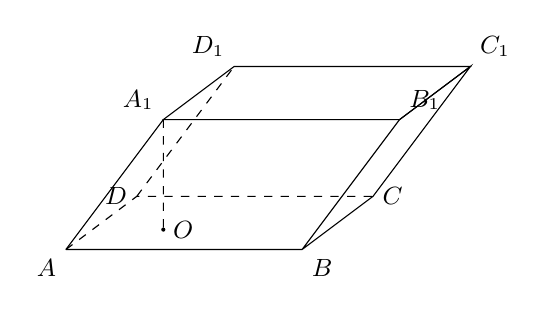
\begin{tikzpicture}[scale=0.75,font=\small]
  \coordinate (A) at (0,0);
  \coordinate (B) at (4,0);
  \coordinate (D) at (1.2,0.9);
  \coordinate (C) at (5.2,0.9);
  \coordinate (A1) at (1.65,2.2);
  \coordinate (B1) at (5.65,2.2);
  \coordinate (D1) at (2.85,3.1);
  \coordinate (C1) at (6.85,3.1);
  \coordinate (O) at (1.65,0.3375);
  \draw (A)--(B)--(C)--(C1)--(B1)--(B) (A)--(A1);
  \draw (A1)--(B1)--(C1)--(D1)--cycle;
  \draw[dashed] (A)--(D)--(C) (D)--(D1) (A1)--(O);
  \fill (O) circle (1pt) node[right] {$O$};
  \node[below left] at (A) {$A$};
  \node[below right] at (B) {$B$};
  \node[right] at (C) {$C$};
  \node[left] at (D) {$D$};
  \node[above left] at (A1) {$A_1$};
  \node[above right] at (B1) {$B_1$};
  \node[above right] at (C1) {$C_1$};
  \node[above left] at (D1) {$D_1$};
\end{tikzpicture}
